% #####################################################################
% #####################################################################
% ##                                                                 ##
% ##                             Lizenz:                             ##
% ##                         CC BY-NC-SA 3.0                         ##
% ##      http://creativecommons.org/licenses/by-nc-sa/3.0/de/       ##
% ##                                                                 ##
% #####################################################################
% ##   Diese Datei kann beliebig verändert werden, solange darauf    ##
% ##     hingewiesen wird, dass dieses Dokument ursprünglich von     ##
% ##                                                                 ##
% ##                        www.ei-studium.de                        ##
% ##                                                                 ##
% ##                             stammt.                             ##
% ## Dies gilt insbesondere auch für alle daraus erstellten Dateien. ##
% ##    Des Weiteren muss die Weitergabe dieser Dateien unter der    ##
% ##                    gleichen Lizenz erfolgen.                    ##
% #####################################################################
% #####################################################################
\documentclass[a4paper,twocolumn,10pt]{article}
\usepackage[utf8]{inputenc}
\usepackage[ngerman]{babel}
\usepackage[top=2.0cm,bottom=1.5cm,left=1.0cm,right=1.0cm]{geometry}
\usepackage{enumitem}
\usepackage{graphicx}
\usepackage{amsfonts}
\usepackage{amsmath}
\usepackage{sectsty}
\usepackage{colortbl}
\usepackage{cancel}
\usepackage{listings}
\usepackage{color}
\usepackage{amsmath}
\usepackage{trfsigns}
\usepackage{epstopdf}
\usepackage{fancyhdr}
\usepackage[pdfborder={0 0 0}]{hyperref}

\setlist{itemsep=.01mm}
\setenumerate{label=\emph{\arabic*})}
\setlength{\columnsep}{1cm}
\parindent 0mm

\partfont{\Large}
\sectionfont{\large \sc\bf}
\subsectionfont{\normalsize}
\subsubsectionfont{\small\textit}

\pagestyle{fancy}
\lhead[\leftmark]{Formelsammlung Mathematik 3 für EI}
\chead[\leftmark]{\url{http://www.ei-studium.de}}
\rhead[\leftmark]{Erstelldatum: \today}
\lfoot[\leftmark]{Keine Garantie auf Vollständigkeit und Richtigkeit!}
\cfoot[\leftmark]{}
\rfoot[\leftmark]{\thepage}
\renewcommand{\headrulewidth}{0.5pt}
\renewcommand{\footrulewidth}{0.5pt}

\begin{document}
\tableofcontents
\newpage

\part{Mathematik 3}

\section{Integration in mehreren Variablen}

\subsection{Allgemeine Rechenregel (Linearität)}
\begin{equation*}
\int\limits_{w}(\alpha f+\beta g)ds=\alpha\int\limits_{w}f\;ds+\beta\int\limits_{w} g\;ds
\end{equation*}

\subsection{Kurvenintegrale / Wegintegrale}

\subsubsection{Wegintegral über stetiges Skalarfeld}
Sei $D\subset\mathbb{R}^n$ offen, $w:I=[a,b]\rightarrow D$ eine differenzierbare Kurve und $f:D\rightarrow\mathbb{R}$ ein stetiges Skalarfeld, dann heißt
\begin{equation*}
\int\limits_{w}f(s)ds=\int\limits_{a}^{b}f(w(t)) \underbrace{||w'(t)||dt}_{ds}
\end{equation*}
das \textbf{Kurvenintegral} von $f$ entlang von $w$.

\subsubsection{Wegintegral über stetiges Vektorfeld}
Sei $E\subset\mathbb{R}^n$ offen, $w:I=[a,b]\rightarrow D$ eine differenzierbare Kurve und $v:D\rightarrow\mathbb{R}^n$ ein stetiges Vektorfeld, dann heißt
\begin{equation*}
\int\limits_{w}v(x)dx=\int\limits_{a}^{b}v(w(t)) \underbrace{\underbrace{T(t)||w'(t)||}_{w'(t)}dt}_{dx}
\end{equation*}
das \textbf{Kurvenintegral} von $v$ entlang von $w$.\\\\
mit dem Tangenteneinheitsvektor
\begin{equation*}
T(t)=\frac{1}{||w'(t)||}w'(t)
\end{equation*}

\subsubsection{Potentialfelder (Gradientenfelder)}
\textbf{Definitionen:}
\begin{enumerate}[label=$\bullet$]
\item Eine Menge $D\subset\mathbb{R}^n$ heißt \textbf{wegzusammenhängend}, falls es zu je zwei Punkten $x,y$ aus $D$ eine Kurve $w:[a,b]\rightarrow D$ mit $w(a)=x$ und $w(b)=y$ gibt.
\item Eine wegzusammenhängende Menge $D\subset\mathbb{R}^n$ heißt \textbf{einfach zusammenhängend}, wenn jede geschlossene doppelpunktfreie Kurve in $D$ stetig auf einen Punkt in $D$ zusammengezogen werden kann, ohne dass $D$ verlassen wird.
\item $G\subseteq\mathbb{R}^n$ heißt \textbf{Gebiet}, falls $G$ offen und zusammenhängend ist.
\item $G\subseteq\mathbb{R}^n$ heißt \textbf{konvex}, falls mit je zwei Punkten $p,q\in G$ auch die Strecke zwischen $p$ und $q$ ganz in $G$ liegt.
\item Sei $C\in\mathbb{R}^n$ eine offene und wegzusammenhängende Menge. Ein stetiges Vektorfeld $f:D\rightarrow\mathbb{R}^n$ heißt \textbf{konservativ}, \textbf{Potentialfeld} oder \textbf{Gradientenfeld}, wenn es ein Skalarfeld $F:D\rightarrow\mathbb{R}$ gibt mit
\begin{equation*}
f(x)=\nabla F(x)\;f\ddot{u}r\;alle\;x\in D
\end{equation*}
In diesem Fall heißt $F$ \textbf{Stammfunktion} und $U=-F$ eine \textbf{Potentialfunktion} von $f$.
\end{enumerate}
Sei $D\subset\mathbb{R}^n$ eine wegzusammenhängende offene Menge und sei $f:D\rightarrow\mathbb{R}^n$ ein stetiges Vektorfeld, dann sind folgende Aussagen äquivalent:
\begin{enumerate}[label=$\bullet$]
\item $f$ ist ein Gradientenfeld
\item Für alle stetig differenzierbaren Kurven $w$ in $D$ hängt das Kurvenintegral $\int\limits_{w}f\;dx$ nur vom Anfangs- und Endpunkt von $w$ ab.
\item Für alle geschlossenen stetig differenzierbaren Kurven $w$ in $D$ gilt
\begin{equation*}
\oint\limits_{w} f\;dx=0
\end{equation*}
\end{enumerate}
\textbf{Überprüfung auf Gradientenfeld:}\\
Sei $D\subset\mathbb{R}^n$ eine offene, einfach zusammenhängende Menge und sei $f:D\rightarrow\mathbb{R}^n$ ein stetig differenzierbares Vektorfeld. Dieses Vektorfeld ist genau dann ein Gradientenfeld, wenn die sogenannte \textbf{Integrabilitätsbedingung}
\begin{equation*}
J_f(x)=J_f(x)^T\;f\ddot{u}r\;alle\;x\in D
\end{equation*}
bzw.
\begin{equation*}
\partial_{x_i}f_j(x)=\partial_{x_j}f_i(x)\;f\ddot{u}r\;alle\;1\leq i,j\leq n
\end{equation*}
oder
\begin{equation*}
rot(f(x))=0\;f\ddot{u}r\;alle\;x\in D\;im\;\mathbb{R}^3
\end{equation*}
erfüllt ist.\\\\
\textbf{Hauptsatz über Kurvenintegrale:}\\
Sei $G\subset\mathbb{R}^n$ Gebiet, $v:G\rightarrow\mathbb{R}^n$ stetiges Gradientenfeld mit Stammfunktion $F$, dann gilt für jede stückweise reguläre Kurve $w$:
\begin{equation*}
\int\limits_{w}v\;dx=F(w(b))-F(w(a))
\end{equation*}
\textbf{Berechnung einer Stammfunktion} (hier im $\mathbb{R}^3$):\\\\
Sei $v(x_1,x_2,x_3)=\begin{pmatrix}v_1(x_1,x_2,x_3) \\ v_2(x_1,x_2,x_3) \\ v_3(x_1,x_2,x_3)\end{pmatrix}$ das Gradientenfeld.\\
Dann berechnet sich die Stammfunktion wie folgt:
\begin{enumerate}
\item $v_1$ nach $x_1$ integrieren\\
$\Rightarrow$ Integrationskostante $C(x_2,x_3)$
\item Das Ergebnis $F$ der Integration partiell nach $x_2$ ableiten und mit $v_2$ gleichsetzen $\Rightarrow$ Gleichung für $\partial_{x_2}C(x_2,x_3)$ in der $x_1$ herausfallen muss.
\item Gleichung $C_{x_2}(x_2,x_3)=...$ nach $x_2$ integrieren\\
$\Rightarrow$ $C(x_2,x_3)=...+C(x_3)$
\item Ergebnis in $F$ einsetzen und partiell nach $x_3$ ableiten...
\end{enumerate}

\subsection{Mehrfachintegration über Skalarfeld entlang von Koordinatenlinien}

\subsubsection{Allgemein}
\textbf{Definitionen:}
\begin{enumerate}[label=$\bullet$]
\item $B\subseteq\mathbb{R}^n$ heißt kompakt oder \textbf{Kompaktum}, falls $B$ abgeschlossen und beschränkt ist.
\item Sei $B\subseteq\mathbb{R}^n$ Kompaktum. $B$ heißt \textbf{messbar}, falls $F=\int\limits_{B}1\;dV$ existiert.
\item Ein Kompaktum $B\subseteq\mathbb{R}^n$ heißt \textbf{Nullmenge}, falls $F(B)=0$
\item Kompaktum $B\subseteq\mathbb{R}^n$ messbar $\Leftrightarrow\;\partial B$ ist Nullmenge
\end{enumerate}
\textbf{Satz:}\\
Jedes $f\in C^1(B)$ auf einem messbaren Kompaktum $B\subseteq\mathbb{R}^n$ ist integrierbar.\\\\
\textbf{Mittelwertsatz:}\\
Sei $f$ integrierbar über einem messbaren Kompaktum $B\subseteq\mathbb{R}^n$. Sei $m=\inf\limits_{x\in B}(f),M=\sup\limits_{x\in B}(f)$.\\
Dann gilt
\begin{equation*}
m\cdot F(B)\leq\int\limits_{B}f\;dx\leq M\cdot F(B)
\end{equation*}
Falls $B$ zusammenhängend, dann existiert ein $(x_1,...,x_n)\in B$, sodass gilt:
\begin{equation*}
\int\limits_{B}f\;dx=f(x_1,...,x_n)\cdot F(B)
\end{equation*}

\subsubsection{Integration über Normalbereich}
Der \textbf{Normalbereich} $B$ ist wie folgt definiert:
\begin{equation*}
\begin{split}B=\{(x_1,x_2,...,x_n)^T:g_1\leq x_1\leq h_1\land g_2(x_1)\leq x_2\leq h_2(x_1)\\ \land...\land g_n(x_1,...,x_{n-1})\leq x_n\leq h(x_1,...,x_{n-1})\}\end{split}
\end{equation*}
mit $f:B\rightarrow\mathbb{R}$ und $g,h$ stetig.\\\\
Das Integral von $f$ über $B$ berechnet sich dann wie folgt:
\begin{equation*}
\int\limits_{B}f\;dx=\int\limits_{g_1}^{h_1}\int\limits_{g_2(x_1)}^{h_2(x_1)}...\int\limits_{g_n(x_1,...,x_{n-1})}^{h_n(x_1,...,x_{n-1})}f(x_1,...,x_{n})dx_n...dx_1
\end{equation*}

\subsubsection{Koordinatentransformation im $\mathbb{R}^n$}
\textbf{Voraussetzungen:}
\begin{enumerate}[label=$\bullet$]
\item $G$ und $G^*$ sind Gebiete im $\mathbb{R}^n$
\item $T:G^*\rightarrow G$ bijektiv und stetig differenzierbar
\item $det(J_T(u))\neq 0\;\forall u\in G^*$
\end{enumerate}
Es gilt:
\begin{equation*}
T(u)=\begin{pmatrix}x_1 \\ \vdots \\ x_n\end{pmatrix}=\begin{pmatrix}g_1(u_1,...,u_n) \\ \vdots \\ g_n(u_1,...,u_n)\end{pmatrix}
\end{equation*}
Die Funktionalmatrix von $T:G^*\rightarrow G$ lautet dann:
\begin{equation*}
J_T(u)=\begin{pmatrix}\frac{\partial g_1}{\partial u_1} & ... & \frac{\partial g_1}{\partial u_n} \\ \vdots & \ddots & \vdots \\ \frac{\partial g_n}{\partial u_1} & ... & \frac{\partial g_n}{\partial u_n}\end{pmatrix}
\end{equation*}
Die Funktionaldeterminante ist definiert als
\begin{equation*}
\frac{\partial (x_1,...,x_n)}{\partial (u_1,...,u_n)}=det(J_T)
\end{equation*}
\textbf{Zylinderkoordinaten:}\\
Mit $0\leq r, 0\leq \varphi\leq 2\pi$ gilt
\begin{equation*}
T(r,\varphi,z)=\begin{pmatrix}x \\ y \\ z\end{pmatrix}=\begin{pmatrix}r\cdot cos(\varphi) \\ r\cdot sin(\varphi) \\ z\end{pmatrix}
\end{equation*}
\begin{equation*}
\frac{\partial (x,y,z)}{\partial (r,\varphi,z)}=r
\end{equation*}
\textbf{Kugelkoordinaten:}\\
Mit $0\leq r,0\leq \varphi\leq 2\pi,-\frac{\pi}{2}\leq \theta\leq\frac{\pi}{2}$ gilt
\begin{equation*}
T(r,\varphi,\theta)=\begin{pmatrix}x \\ y \\ z\end{pmatrix}=\begin{pmatrix}r\cdot cos(\varphi)cos(\theta) \\ r\cdot sin(\varphi)cos(\theta) \\ r\cdot sin(\theta)\end{pmatrix}
\end{equation*}
\begin{equation*}
\frac{\partial (x,y,z)}{\partial (r,\varphi,\theta)}=r^2cos(\theta)
\end{equation*}
\textbf{Elliptische Koordinaten}\\
Mit $0\leq r, 0\leq \varphi\leq 2\pi$ gilt
\begin{equation*}
T(r,\varphi)=\begin{pmatrix}x \\ y \end{pmatrix}=\begin{pmatrix}a\cdot r\cdot cos(\varphi) \\ b\cdot r\cdot sin(\varphi)\end{pmatrix}
\end{equation*}
\begin{equation*}
\frac{\partial (x,y)}{\partial (r,\varphi)}=a\cdot b\cdot r
\end{equation*}
\textbf{Komposition von Transformationen:}\\
Es gilt
\begin{equation*}
det(J_S\circ J_T)=det(J_S)\cdot det(J_T)
\end{equation*}
\textbf{Transformationsformel:}\\
Sei $B^*$ eine messbare kompakte Teilmenge von $G^*$, dann gilt
\begin{equation*}
\int\limits_{B}f(x)\;dx=\int\limits_{B^*}f(T(u))|det(J_T)|du
\end{equation*}

\subsection{Parameterabhängige Integrale}
Sei $t\in I\subseteq \mathbb{R}, f:B\subseteq\mathbb{R}^n\rightarrow\mathbb{R}$, wobei $f$ für jedes festgehaltene $t$ integrierbar sein muss und sei
\begin{equation*}
F(t)=\int\limits_{B}f(x,t)dx
\end{equation*}
Dann ist auch $F$ in $I$ stetig.\\
Seien $f\in C^1(B\times I),\frac{\partial f}{\partial t}\in C(B\times I)$, dann ist $F\in C^1$ und es gilt:
\begin{equation*}
\frac{dF}{dt}=\int\limits_{B}\frac{df(x,t)}{dt}dx=\frac{d}{dt}\int\limits_{B}f(x,t)dx
\end{equation*}

\subsubsection{Variable Integrationsgrenzen}
Sei $t\in I\subseteq\mathbb{R}$, sei $B\subseteq\mathbb{R}^n$ ein Bereich, der alle Punkte $(x,t)$ enthält, für die $\varphi(t)\leq x\leq \psi(t)$ gilt, sei $\varphi,\psi\in C^1(I), f\in C^1(B),\frac{\partial f}{\partial t}\in C(B)$ und sei
\begin{equation*}
F(t)=\int\limits_{\varphi(t)}^{\psi(t)}f(x,t)dx
\end{equation*}
dann existieren $\frac{\partial F}{\partial t},\frac{\partial F}{\partial\varphi}$ und $\frac{\partial F}{\partial \psi}$ und es gilt
\begin{equation*}
\frac{dF}{dt}=\frac{\partial F}{\partial t}+\underbrace{\frac{\partial F}{\partial \varphi}}_{-f(\varphi(t),t)}\cdot\frac{d\varphi}{dt}+\underbrace{\frac{\partial F}{\partial\psi}}_{f(\psi(t),t)}\cdot\frac{d\psi}{dt}
\end{equation*}
\textbf{Leibniz-Regel:}\\
\begin{equation*}
\frac{dF}{dt}=\int\limits_{\varphi(t)}^{\psi(t)}\frac{\partial f(x,t)}{\partial t}dx-f(\varphi(t),t)\frac{d\varphi}{dt}+f(\psi(t),t)\frac{d\psi}{dt}
\end{equation*}

\subsection{Flächenintegrale}

\subsubsection{Flächenstück}
Sei $D\subseteq\mathbb{R}^2$ offen und messbar, $f:\overline{D}\rightarrow\mathbb{R}^3,f\in C^1(\overline{D})$ und gelte $Rang(f')=2\;\forall (u,v)^T\in D$.\\
Dann heißt $f(\overline{D})$ Flächenstück $F$ im $\mathbb{R}^3$.\\
Sei
\begin{equation*}
f_u=\frac{\partial f}{\partial u}=\begin{pmatrix}\partial_u X \\ \partial_u Y \\ \partial_u Z\end{pmatrix};\;\;f_v=\frac{\partial f}{\partial v}=\begin{pmatrix}\partial_v X \\ \partial_v Y \\ \partial_v Z\end{pmatrix}
\end{equation*}
\begin{equation*}
f'(u,v)=J_f(u,v)=\begin{pmatrix}\partial_u X & \partial_v X \\ \partial_u Y & \partial_v Y \\ \partial_u Z & \partial_v Z\end{pmatrix}
\end{equation*}
Falls $Rang(f')=2$:
\begin{equation*}
\Rightarrow f_u,f_v\;linear\;unabh\ddot{a}ngig\Leftrightarrow f_u\times f_v\neq 0
\end{equation*}

\subsubsection{Tangentialebene von $F$ im Punkt $(x_0,y_0,z_0)^T$}
Die Tangentialebene wird für $\lambda,\mu\in\mathbb{R}$ wie folgt beschrieben:
\begin{equation*}
\begin{pmatrix}x \\ y \\z\end{pmatrix}=\begin{pmatrix}x_0 \\ y_0 \\ z_0\end{pmatrix}+J_f(u_0,v_0)\cdot\begin{pmatrix}\lambda \\ \mu\end{pmatrix}
\end{equation*}
bzw.
\begin{equation*}
\begin{pmatrix}x \\ y \\z\end{pmatrix}=\begin{pmatrix}x_0 \\ y_0 \\ z_0\end{pmatrix}+\lambda f_u(u_0,v_0)+\mu f_v(u_0,v_0)
\end{equation*}

\subsubsection{Tangentialvektor von $\hat{K}$ im Punkt $(x_0,y_0,z_0)^T$}
Sei
\begin{equation*}
K:\begin{pmatrix}u \\ v\end{pmatrix}=\gamma(t)=\begin{pmatrix}\gamma_1(t) \\ \gamma_2(t)\end{pmatrix}
\end{equation*}
und sei
\begin{equation*}
\hat{K}:\begin{pmatrix}x \\ y \\ z\end{pmatrix}=k(t)=f(\gamma(t))
\end{equation*}
Dann wird der Tangentialvektor von $\hat{K}$ an der Stelle $(x_0,y_0,z_0)^T \in F$ wie folgt beschrieben:
\begin{equation*}
\dot{x}(t)=J_f(\gamma(t)) \dot{\gamma}(t)\in\;Tangentialebene
\end{equation*}
\subsubsection{Einheitsnormalenvektor}
Für $x_0=f(u_0,v_0)\in F$ gilt
\begin{equation*}
n(x_0)=\frac{f_u(x_0)\times f_v(x_0)}{|f_u(x_0)\times f_v(x_0)|};\;\;n\perp\;Tangentialebene
\end{equation*}

\subsubsection{Parametertransformationen}
\textbf{Definitionen:}
\begin{enumerate}[label=$\bullet$]
\item $\varphi:\overline{D}\rightarrow\overline{G}$ heißt \textbf{Diffeomorphismus}, wenn $\varphi\in C^1(\overline{D})$, $\varphi$ eindeutig umkehrbar (bijektiv) und $\varphi^{-1}\in C^1(\overline{G})$
\item Sei $F$ ein Flächenstück. Die Parameterdarstellung $g:\overline{G}\rightarrow\mathbb{R}$ von $F$ heißt \textbf{äquivalent} zur Parameterdarstellung $f:\overline{D}\rightarrow\mathbb{R}$ von $F$ (kurz $g\sim f$), wenn $g=f\circ \varphi$ gilt, wobei $\varphi$ ein Diffeomorphismus mit $det(\varphi')>0$ ist.
\item Ein Flächenstück heißt \textbf{doppelpunktfrei} (injektiv), falls $f:\overline{D}\rightarrow\mathbb{R}^3$ injektiv ist.\\
Alle doppelpunktfreien Flächen haben genau 2 Orientierungen.
\item Eine \textbf{Fläche} ist eine Vereinigung endlich vieler injektiver Flächenstücke, wobei je zwei Flächenstücke höchstens Randpunkte gemeinsam haben.
\end{enumerate}

\subsubsection{Flächenintegral}
Sei $F:f:\overline{D}\rightarrow\mathbb{R}^3$ ein injektives Flächenstück. Dann gilt
\begin{equation*}
A(F)=\int\int\limits_{F}dA=\int\int\limits_{\overline{D}}|f_u\times f_v|dudv
\end{equation*}
\textbf{Grundlegende Eigenschaften:}\\
Seien $F,\hat{F}$ disjunkt, dann gilt
\begin{enumerate}[label=$\bullet$]
\item Additivität: $A(F\cup\hat{F})=A(F)+A(\hat{F})$
\item Monotonie: $F\subseteq \hat{F}\Rightarrow A(F)\leq A(\hat{F})$
\item Bewegungsinvarianz:\\
Sei $\beta$ Bewegung (Translation, Rotation, Spiegelung)\\
$\Rightarrow A(\beta(F))=A(F)$
\item Normierung: $Q=[0,1]\times [0,1]\times \{0\}: A(Q)=1$
\end{enumerate}

\subsubsection{Flächenintegral 1. Art}
Sei $F:f:\overline{D}\rightarrow\mathbb{R}^3$ ein injektives Flächenstück, $F\subseteq A\subseteq\mathbb{R}^3$ und sei $G:A\rightarrow\mathbb{R}$ stetig, dann gilt
\begin{equation*}
\int\int\limits_{F}G\;dA=\int\int\limits_{\overline{D}}G(f(u,v))||f_u\times f_v||dudv
\end{equation*}

\subsubsection{Flächenintegral 2. Art}
Sei $F:f:\overline{D}\rightarrow\mathbb{R}^3$ ein injektives Flächenstück, $F\subseteq A\subseteq\mathbb{R}^3$ und sei $v:A\supseteq F\rightarrow\mathbb{R}^3$ ein stetiges Vektorfeld, dann gilt
\begin{equation*}
\int\int\limits_{F}G\;d\sigma=\int\int\limits_{\overline{D}}v(f(u,v))\underbrace{(f_u\times f_v)dudv}_{d\sigma}
\end{equation*}
\begin{equation*}
d\sigma =\underbrace{\frac{f_u\times f_v}{||f_u\times f_v||}}_{n_F}\underbrace{||f_u\times f_v||dudv}_{dA}
\end{equation*}

\subsubsection{Transformationsformel für Flächenintegrale 2. Art}
Sei $F:f:\overline{D}\rightarrow\mathbb{R}^3$ ein injektives Flächenstück, $F\subseteq A\subseteq\mathbb{R}^3$, sei $v:A\supseteq F\rightarrow\mathbb{R}^3$ ein stetiges Vektorfeld und sei $S:\mathbb{R}^3\rightarrow\mathbb{R}^3$ ein Diffeomorphismus mit
\begin{equation*}
F^*:x^*=S(x)=S(f(u,v))
\end{equation*}
dann gilt
\begin{equation*}
\int\int\limits_{F}v\;d\sigma =\int\int\limits_{F^*}v^*\;d\sigma^*
\end{equation*}
mit
\begin{equation*}
v^*(x^*)=\frac{J_S(S^{-1}(x^*))}{det(J_S(S^{-1}(x^*)))}\cdot v(S^{-1}(x^*))
\end{equation*}

\subsection{Integralsätze}
\textbf{Definition (Bereich):}\\
Sei $B\subseteq\mathbb{R}^3$ kompakt. $B$ heißt \textbf{Bereich} mit \textbf{stückweise glattem Rand}, wenn $B=\overline{B}_0$ ($B_0\subseteq\mathbb{R}^3$ offen) und $\partial B=\bigcup\limits_{i=1}^{n}F_i$, wobei $F_i$ Flächenstücke sind.

\subsubsection{Integralsatz von Gauß}
Sei $B\subseteq\mathbb{R}^3$ ein Bereich mit stückweise glattem Rand und sei $v\in C^1(B)$ ein Vektorfeld, dann gilt
\begin{equation*}
\int\limits_{\partial B}v\;d\sigma =\int\limits_{B}div(v)dV
\end{equation*}

\subsubsection{Integralsatz von Gauß im $\mathbb{R}^2$}
Sei $D$ ein beschränktes Gebiet im $\mathbb{R}^2$ mit stückweise glattem Rand (stückweise $C^1$-Kurve) $K:\gamma=(\gamma_1,\gamma_2)^T, \gamma:[a,b]\rightarrow\mathbb{R}^2$ und sei $v:D\rightarrow\mathbb{R}^2$ ein $C^1$-Vektorfeld, dann berechnet sich der Fluss $v$ \underline{durch} den Rand wie folgt:
\begin{equation*}
\oint\limits_{K}v^T\cdot n\;ds=\int\int\limits_{\overline{D}}div(v)dF
\end{equation*}
\begin{equation*}
\int\limits_{a}^{b}v(\gamma(t))\underbrace{\begin{pmatrix}\dot{\gamma}_2(t) \\ -\dot{\gamma}_1(t)\end{pmatrix}dt}_{n\underbrace{||\dot{\gamma}(t)||dt}_{ds}}=\int\int\limits_{\overline{D}}\left(\frac{\partial v_1}{\partial x_1}+\frac{\partial v_2}{\partial x_2}\right)dF
\end{equation*}
\textbf{Leibnizsche Sektorformel:}
\begin{equation*}
F(G)=\frac{1}{2}\int\limits_{a}^{b}\gamma_1(t)\dot{\gamma_2}(t)-\gamma_2(t)\dot{\gamma_1}(t)dt
\end{equation*}

\subsubsection{Integralsatz von Green im $\mathbb{R}^2$}
Seien die Bedingungen wie zuvor, dann berechnet sich der Fluss $v$ \underline{entlang} des Randes wie folgt:
\begin{equation*}
\oint\limits_{K}v^Tdx=\int\int\limits_{\overline{D}}\left(\frac{\partial v_2}{\partial x_1}-\frac{\partial v_1}{\partial x_2}\right)dF
\end{equation*}
$\underline{\mathcal{N.B.}}$\\
Gauß'scher und Green'scher Satz gelten auch für Gebiete $G=\bigcup\limits_{i=1}^{n}D_i$

\subsection{1. Green'sche Formel}
Sei $B\subseteq\mathbb{R}^3$ ein Kompaktum mit abschnittsweise glattem Rand und seien $\varphi\in C^1(B)$ ein Skalarfeld und $v\in C^1(G)$ ein Vektorfeld, dann gilt
\begin{equation*}
\int\int\limits_{\partial B}\varphi\cdot v\;d\sigma=\int\limits_{B}(\nabla\varphi\cdot v+\varphi\cdot \nabla v)dV
\end{equation*}

\subsubsection{Gauß'scher Satz für Skalarfelder}
\textbf{Definition:}\\
$B\subseteq\mathbb{R}^3$ heißt \textbf{Gauß'scher Bereich}, wenn für alle $v\in C^1(B)$ der Gauß'sche Integralsatz gilt.\\\\
Sei $B:$ Gauß'scher Bereich, $\varphi\in C^1(B)$ ein Skalarfeld, dann gilt
\begin{equation*}
\int\int\limits_{\partial B}\varphi\cdot \underbrace{n\cdot dA}_{d\sigma}=\int\limits_{B}\nabla\varphi dV
\end{equation*}

\subsubsection{Satz von Stokes}
Sei $F:$ stückweise glatt berandet, $v\in C^1(M), F\subseteq M\subseteq\mathbb{R}^3$, dann gilt
\begin{equation*}
\oint\limits_{\partial F}v\;dx=\int\int\limits_{F}rot(v)d\sigma
\end{equation*}
\textbf{Folgerung:}\\
Sei $M\subseteq\mathbb{R}^3$ und $B\subseteq M$ ein Gauß'scher Bereich mit stückweise glattem Rand, dann gilt
\begin{equation*}
\int\int\limits_{\partial B}rot(v)d\sigma=0
\end{equation*}
$\mathcal{N.B.}$\\
Im $\mathbb{R}^2$ gilt: "Green = Gauß = Stokes"

\subsection{Vektorpotential}
\textbf{Definition:}\\
$G\subseteq\mathbb{R}^n$ heißt \textbf{sternförmig}, wenn ein $x_0\in G$ existiert, sodass jeder andere Punkt $x\in G$ sich geradlinig in $G$ mit $x_0$ verbinden lässt.\\\\
\textbf{Satz:}\\
Sei $G\subseteq\mathbb{R}^3$ sternförmig und $v\in C^1(G)$, dann gilt:
\begin{equation*}
div(v)=0\Leftrightarrow \exists\;a\in C^1(G): v=rot(a)
\end{equation*}
Das Vektorpotential berechnet sich dann wie folgt:
\begin{equation*}
a(x)=\int\limits_{0}^{1}t\cdot v(x_0+t(x-x_0))\times (x-x_0)dt
\end{equation*}
Alle Vektorpotentiale von $v$ haben die Form
\begin{equation*}
a+grad(\varphi)
\end{equation*}
wobei $\varphi\in C^2(G)$ ein beliebiges Skalarfeld ist.

\subsection{Helmholtz'scher Zerlegungssatz}
Sei $G$ ein beschränktes Gebiet im $\mathbb{R}^3$ und $v\in C^2(G)$, dann existiert ein $\varphi\in C^1(G)$ und ein $a\in C^1(G)$, sodass gilt:
\begin{equation*}
v=\nabla\varphi+rot(a)
\end{equation*}

\section{Integraltransformationen}

\subsection{Grundlagen}

\subsubsection{Skalarprodukt}
Sei $V$ ein Vektorraum über $\mathbb{C}$.\\
Eine Abbildung $(x,y)\in V\times V\rightarrow\langle x,y\rangle \in\mathbb{C}$ ist ein Skalarprodukt, falls für alle $x,y,z\in V$ und $\alpha\in\mathbb{C}$ gilt:
\begin{enumerate}
\item $\langle x,x\rangle >0\;\forall x\neq 0$ und $\langle 0,0\rangle=0$
\item $\langle\alpha x,y\rangle =\alpha\langle x,y\rangle$\\
$\langle x,\alpha y\rangle =\overline{\alpha}\langle x,y\rangle$
\item $\langle x+y,z\rangle =\langle x,z\rangle+\langle y,z\rangle$\\
$\langle x,y+z\rangle =\langle x,y\rangle +\langle x,z\rangle$
\item $\langle x,y\rangle=\overline{\langle y,x\rangle}$
\end{enumerate}
\textbf{Eigenschaften:}\\
\begin{enumerate}
\item Skalarprodukt ist Orthogonalitätsmaß
\begin{equation*}
x\perp y\text{, falls }\langle x,y\rangle=0
\end{equation*}
\item Zugehörige Norm
\begin{equation*}
||x||=||x||_v=\sqrt{\langle x,x\rangle}
\end{equation*}
\item Seien $v_1,...,v_m\in V$ orthogonal, d.h. $\langle v_i,v_j\rangle=0$ für $i\neq j$, dann gilt
\begin{equation*}
||v_1+...+v_m||^2=||v_1||^2+...+||v_m||^2
\end{equation*}
\item Seien $v_1,...,v_m\in V$ orthonormal, d.h. $\langle v_i,v_j\rangle=\delta_{ij}$, dann gilt für $\gamma_1,...,\gamma_m\in\mathbb{C}$
\begin{equation*}
||\gamma_1 v_1+...+\gamma_m v_m||^2=|\gamma_1|^2+...+|\gamma_m|^2
\end{equation*}
\item Cauchy-Schwarz-Ungleichung
\begin{equation*}
|\langle x,y\rangle|\leq||x||\cdot||y||\;\forall x,y\in V
\end{equation*}
\end{enumerate}

\subsubsection{Hilbertraum}
\textbf{Definition:}\\
Ein Vektorraum $H$ mit Skalarprodukt, der vollständig (d.h. jede Cauchy-Folge konvergiert in $H$) ist, heißt \textbf{Hilbertraum}.

\subsubsection{Orthonormalsystem}
\textbf{Definition:}\\
Sei $H$ ein Hilbertraum.\\
Ein System $(e_{ij})_{j\in I}$ mit $e_j\in H$ heißt \textbf{Orthonormalystem (ONS)}, falls
\begin{equation*}
\langle e_i,e_j\rangle =\delta_{ij}\;\;\;\;\;\forall i,j\in I
\end{equation*}
und \textbf{vollständig}, falls
\begin{equation*}
x=\sum\limits_{j\in I}\langle x,e_j\rangle e_j\;\;\;\;\;\forall x\in H
\end{equation*}
\textbf{Lemma:}\\
Sei $H$: Hilbertraum und $(e_j){j\in I}$ ein vollständiges ONS, dann gilt für die \textbf{orthogonale Projektion $S_N$} (Fourier-Summe):
\begin{equation*}
S_N=\sum\limits_{|j|\leq N}\langle x,e_j\rangle e_j
\end{equation*}
und
\begin{equation*}
(x-S_N)\perp span\{e_j:|j|\leq N\}
\end{equation*}
Somit gilt
\begin{equation*}
||x||^2=||S_N||^2+||x-S_N||^2
\end{equation*}
und insbesondere die Bessel'sche Ungleichung:
\begin{equation*}
||x||^2\geq ||S_N||^2
\end{equation*}

\subsubsection{Dirac-Distribution - Rechenregeln}
\begin{enumerate}[label=$\bullet$]
\item $\int\limits_{-\infty}^{\infty}f(t)\delta (t-t_0)dt=f(t_0)$
\item $\delta (t)=\frac{1}{2\pi}\int\limits_{-\infty}^{\infty}e^{\pm i\omega t}d\omega;\;\;\delta (\omega)=\frac{1}{2\pi}\int\limits_{-\infty}^{\infty}e^{\pm i\omega t}dt$
\item $\delta(at)=\frac{\delta (t)}{|a|}$
\item $\frac{1}{T_0}\sum\limits_{k=-\infty}^{\infty}e^{ik\omega_0 t}=\sum\limits_{n=-\infty}^{\infty}\delta(t-nT_0)$
\item $\sum\limits_{n=-\infty}^{\infty}e^{-in\omega T_0}=\omega_0\sum\limits_{k=-\infty}^{\infty}\delta(\omega-k\omega_0)$
\item $f(t)*\delta(t-t_0)=f(t-t_0)$
\end{enumerate}

\subsubsection{Sonstiges}
\begin{equation*}
sin(x)=\frac{e^{ix}-e^{-ix}}{2i};\;\;\;\;\;\;\;cos(x)=\frac{e^{ix}+e^{-ix}}{2}
\end{equation*}

\subsection{Fourier-Reihe}
Sei $V=\{f:(O,T)\rightarrow\mathbb{C},\text{stückweise stetig}\}$ bzw.\\
$V=\{f:\mathbb{R}\rightarrow\mathbb{C},\text{T-periodisch, stückweise stetig}\}$ und gelte $\alpha,\beta\in\mathbb{C}$, dann ist das Skalarprodukt von $f,g\in V$ wie folgt definiert:
\begin{equation*}
\langle f,g\rangle=\frac{1}{T}\int\limits_{T}f(t)\overline{g(t)}dt
\end{equation*}
\begin{equation*}
||f||^2=\frac{1}{T}\int\limits_{T}|f(t)|^2 dt
\end{equation*}
Die Fourier-Basis (ONS) ist wie folgt definiert:
\begin{equation*}
e_k=e^{ik\omega t}\;\;\;\;\;k\in\mathbb{Z},\;\omega=\frac{2\pi}{T}
\end{equation*}

\subsubsection{Fourier-Analyse}
Bei der Fourier-Analyse wird der Zeitbereich in ein Frequenzbereich (Spektrum von $f$) überführt.
\begin{equation*}
f\laplace (c_k)_{k\in\mathbb{Z}}=\langle f,e_k\rangle=\frac{1}{T}\int\limits_{T}f(t)e^{-ik\omega t}dt
\end{equation*}
\underline{$\mathcal{N.B.}$}\\
Falls z.B. $T=2\pi$ gewählt wird und die Funktion $f(t)$ sogar $\pi$-periodisch ist, dann gilt $c_k=0$ für alle ungeraden $k$.

\subsubsection{Fourier-Synthese}
Bei der Fourier-Synthese wird der Frequenzbereich in den Zeitbereich überführt.
\begin{equation*}
(c_k)_{k\in\mathbb{Z}}\Laplace f=\sum\limits_{k\in\mathbb{Z}}\langle f,e_k\rangle e_k(t)=\sum\limits_{k\in\mathbb{Z}}c_k e^{ik\omega t}
\end{equation*}

\subsubsection{Reelle Darstellung}
Falls $f$ reellwertig, dann gilt $\overline{c_k}=c_{-k}$.
Die reelle Darstellung lautet wie folgt:
\begin{equation*}
f(t)=\underbrace{\frac{a_0}{2}+\sum\limits_{k=1}^{\infty}a_k\cos(k\omega t)}_{\text{gerader Anteil}}+\underbrace{\sum\limits_{k=1}^{\infty}b_k\sin(k\omega t)}_{\text{ungerader Anteil}}
\end{equation*}
Für die Koeffizienten gilt:
\begin{equation*}
a_k=2Re(c_k)=\frac{2}{T}\int\limits_{T}f(t)\cos(k\omega t)dt
\end{equation*}
\begin{equation*}
b_k=-2Im(c_k)=\frac{2}{T}\int\limits_{T}f(t)\sin(k\omega t)dt
\end{equation*}
\begin{equation*}
c_k=\frac{a_k-ib_k}{2}\text{ für }k>0
\end{equation*}

\subsubsection{Konvergenz von $S_N$}
Sei $f:\mathbb{R}\rightarrow\mathbb{C}$ stückweise stetig diffbar (mit nur endlich vielen Sprungstellen), dann gilt:
\begin{enumerate}[label=$\bullet$]
\item $S_N$ konvergiert für alle $t\in\mathbb{R}$
\item $S_N$ konvergiert gleichmäßig auf jedem abgeschlossenen Intervall ohne Sprungstelle
\item An den Sprungstellen gilt
\begin{enumerate}[label=$\bullet$]
\item $S_f(t)=\frac{f(t^+)+f(t^-)}{2}$
\item Gibbs-Phänomen:\\
$S_N$ schwingt für $N\rightarrow\infty$ stets um ca. $18 \%$ über.
\end{enumerate}
\end{enumerate}

\subsubsection{Rechenregeln}
Seien $f,g:\mathbb{R}\rightarrow\mathbb{C}$ stückweise stetig diffbar und $T$-periodisch, dann gelten für
\begin{equation*}
f\laplace (c_k)_{k\in\mathbb{Z}}\;\;\;\;\;\;\;\;g\laplace (d_k)_{k\in\mathbb{Z}}
\end{equation*}
folgende Rechenregeln:
\begin{enumerate}[label=$\bullet$]
\item Linearität ($\alpha,\beta\in\mathbb{C}$)
\begin{equation*}
\alpha f+\beta g\laplace (\alpha c_k+\beta d_k)_{k\in\mathbb{Z}}
\end{equation*}
\item Konjugation
\begin{equation*}
\overline{f}\laplace (\overline{c_{-k}})_{k\in\mathbb{Z}}
\end{equation*}
\item Zeitumkehr
\begin{equation*}
f(-t)\laplace (c_{-k})_{k\in\mathbb{Z}}
\end{equation*}
\item Änderung der Zeitskala
\begin{equation*}
f(\gamma t)\laplace (c_k)_{k\in\mathbb{Z}};\;\;\;\;\;\gamma>0
\end{equation*}
Periode: $\frac{T}{\gamma}$
\item Verschiebung im Zeitbereich (Phasenverschiebung)
\begin{equation*}
f(t+a)\laplace (e^{ik\omega a}c_k)_{k\in\mathbb{Z}};\;\;\;\;\;a\in\mathbb{R}
\end{equation*}
\item Verschiebung im Spektralbereich
\begin{equation*}
e^{in\omega t}f(t)\laplace (c_{k-n})_{k\in\mathbb{Z}}
\end{equation*}
\item Symmetrien
\begin{enumerate}[label=-]
\item $f$ gerade: $f\left(\frac{T}{2}+t\right)=f\left(\frac{T}{2}-t\right)$
\begin{equation*}
c_k=c_{-k}
\end{equation*}
\begin{equation*}
a_k=\frac{4}{T}\int\limits_{0}^{\frac{T}{2}}f(t)\cos(k\omega t)dt
\end{equation*}
\begin{equation*}
b_k=0
\end{equation*}
\item $f$ ungerade: $f\left(\frac{T}{2}+t\right)=-f\left(\frac{T}{2}-t\right)$
\begin{equation*}
c_k=-c_{-k}
\end{equation*}
\begin{equation*}
a_k=0
\end{equation*}
\begin{equation*}
b_k=\frac{4}{T}\int\limits_{0}^{\frac{T}{2}}f(t)\sin(k\omega t)dt
\end{equation*}
\end{enumerate}
\item Ableitung\\
Sei $f$ stetig, $f'$ stückweise stetig, dann gilt
\begin{equation*}
f'(t)\laplace (i\omega kc_k)_{k\in\mathbb{Z}}
\end{equation*}
\item Stammfunktion\\
Sei $f$ stückweise stetig und $c_0=0$ (sonst ist die Stammfunktion nicht periodisch), dann gilt
\begin{equation*}
F(t)=\int\limits_{0}^{t}f(\tau)d\tau \laplace\begin{cases}\frac{c_k}{ik\omega} & k\in\mathbb{Z}\setminus\{0\} \\ -\frac{1}{T}\int\limits_{0}^{T}tf(t)dt & k=0\end{cases}
\end{equation*}
\item Größenordnung der Fourierkoeffizienten\\
$f,f',...,f^{(m-1)}$ stetig, $f^{(m)}$ stückweise stetig
\begin{equation*}
\exists M>0:|c_k|\leq\frac{M}{|k|^m}
\end{equation*}
Sonderfall: $f\in C^{\infty}$
\begin{equation*}
\Rightarrow \forall m\;\exists M=M(m):|c_k|\leq\frac{M}{|k|^m}
\end{equation*}
\item Periodische Faltung
\begin{equation*}
(f*g)(t)=\frac{1}{T}\int\limits_{T}f(t-\tau)g(\tau)d\tau\laplace (c_kd_k)_{k\in\mathbb{Z}}
\end{equation*}
\end{enumerate}
\subsubsection{Rechenregeln / Eigenschaften von Faltung}
\begin{enumerate}[label=$\bullet$]
\item Kommutativität
\begin{equation*}
f*g=g*f
\end{equation*}
\item Linearität
\begin{equation*}
h*(\alpha f+\beta g)=\alpha(h*f)+\beta(h*g)
\end{equation*}
\item Glättung: $f,g$ stückweise stetig $\Rightarrow f*g$ stetig
\item Symmetrieeigenschaften:
\begin{enumerate}[label=-]
\item gerade Fkt. * gerade Fkt. $\Rightarrow$ gerade Fkt.
\item ungerade Fkt * ungerade Fkt. $\Rightarrow$ gerade Fkt.
\item ungerade Fkt * gerade Fkt. $\Rightarrow$ ungerade Fkt.
\end{enumerate}
\end{enumerate}

\subsubsection{Häufig verwendete Funktionen}
\underline{Sägezahnfunktion:}
\begin{equation*}
f(t)=\frac{1}{2}(\pi-t);\;\;\;\;\;0\leq t\leq 2\pi
\end{equation*}
\begin{equation*}
c_k=\begin{cases}0 & k=0 \\ \frac{1}{2ki} & k\neq 0\end{cases}
\end{equation*}

\subsection{Diskrete Fourier-Transformation}
Es gilt
\begin{equation*}
c_k\approx\frac{1}{n}\sum\limits_{l=0}^{n-1}f_l\cdot \omega_n^{kl}
\end{equation*}
mit $\omega_n=e^{-\frac{2\pi i}{n}}$ und $k=0,1,...,n-1$.\\
In Matrix-Schreibweise lautet die diskrete FT
\begin{equation*}
\underbrace{\begin{pmatrix}c_0 \\ c_1 \\ \vdots \\ c_{n-1}\end{pmatrix}}_{\tilde{c}}=\frac{1}{n}M\underbrace{\begin{pmatrix}f_0 \\ f_1 \\ \vdots \\ f_{n-1}\end{pmatrix}}_{f}
\end{equation*}
mit
\begin{equation*}
M=\begin{pmatrix}1 & 1 & 1 & 1 & ... & 1 \\ 1 & \omega_n & \omega_n^2 & \omega_n^3 & ... & \omega_n^{n-1} \\ 1 & \omega_n^2 & \omega_n^4 & \omega_n^6 & ... & \omega_n^{2\cdot(n-1)} \\ \vdots & \vdots & \vdots & \vdots & \ddots & \vdots \\ 1 & \omega_n^{n-1} & \omega_n^{(n-1)\cdot 2} & \omega_n^{(n-1)\cdot 3} & ... & \omega_n^{(n-1)(n-1)}\end{pmatrix}
\end{equation*}

\subsubsection{Trigonometrische Interpolation}
Aufgabe:\\
Finde zu gegebenen Daten $(t_l,f_l)$ mit $t_l=\frac{2\pi l}{n}, l=0,1,...,n-1$ ein trigonometrisches Polynom mit
\begin{equation*}
p(t)=\sum\limits_{k=0}^{n-1}p_ke^{ikt}
\end{equation*}
sodass $p(t_l)=f_l\;\forall\;l$
\begin{equation*}
\Rightarrow \text{Lösung: }p=\tilde{c}
\end{equation*}
\underline{$\mathcal{N.B.}$}\\
$\frac{1}{\sqrt{n}}M_n$ ist unitär, d.h. $\overline{M_n^T}M_n=nI$
\begin{equation*}
\Rightarrow \left(\overline{M_n^T}\right)^{-1}=\frac{1}{n}M_n
\end{equation*}

\subsection{Fourier-Transformation (FT)}

\subsubsection{Voraussetzungen}
\begin{enumerate}
\item $f$ stückweise stetig diffbar
\item An Sprungstelle gilt: $f(t)=\frac{f(t^+)+f(t^-)}{2}$
\item $\int\limits_{-\infty}^{\infty}|f(t)|dt<\infty$
\end{enumerate}
Unter diesen Voraussetzungen gilt
\begin{enumerate}[label=$\bullet$]
\item $F(\omega)$ ist beschränkt und stetig
\item Formel von Plancherel
\begin{equation*}
\int\limits_{-\infty}^{\infty}|f(t)|^2dt=\frac{1}{2\pi}\int\limits_{-\infty}^{\infty}|F(\omega)|^2d\omega
\end{equation*}
\end{enumerate}

\subsubsection{Analyse}
\begin{equation*}
f(t)\laplace F(\omega)=\int\limits_{-\infty}^{\infty}f(t)e^{-i\omega t}dt
\end{equation*}

\subsubsection{Synthese}
\begin{equation*}
F(\omega)\Laplace f(t)=\frac{1}{2\pi}\int\limits_{-\infty}^{\infty}F(\omega)e^{i\omega t}d\omega
\end{equation*}

\subsubsection{Rechenregeln}
Für $f\laplace F, g\laplace G$ sowie $\alpha,\beta\in\mathbb{C}$ und $c\neq 0$ gelten folgende Rechenregeln:
\begin{enumerate}[label=$\bullet$]
\item Linearität
\begin{equation*}
\alpha f+\beta g\laplace \alpha F+\beta G
\end{equation*}
\item Konjugation
\begin{equation*}
\overline{f}\laplace \overline{F(-\omega)}
\end{equation*}
\item Skalierung
\begin{equation*}
f(ct)\laplace \frac{1}{|c|}F\left(\frac{\omega}{c}\right)
\end{equation*}
\item Verschiebung im Zeitbereich
\begin{equation*}
f(t-a)\laplace e^{-i\omega a} F(\omega)
\end{equation*}
\item Verschiebung im Frequenzbereich
\begin{equation*}
e^{ia t}\laplace F(\omega-a)
\end{equation*}
\item Symmetrien
\begin{enumerate}[label=-]
\item $f$ gerade $\laplace F(\omega)\text{ gerade}$
\item $f$ gerade $\laplace F(\omega)=2\int\limits_{0}^{\infty}f(t)\cos(\omega t)dt$
\item $f$ ungerade $\laplace F(\omega)\text{ ungerade}$
\item $f$ ungerade $\laplace F(\omega)=-2i\int\limits_{0}^{\infty}f(t)\sin(\omega t)dt$\\\\
$\Rightarrow f_g\laplace Re(F(\omega))$ bzw. $f_u\laplace iIm(F(\omega))$
\end{enumerate}
\item Ableitung im Zeitbereich\\
$f'$ erfüllt 1) und 3), $f$ stetig
\begin{equation*}
f'\laplace i\omega F(\omega)
\end{equation*}
\item Ableitung im Frequenzbereich\\
$tf(t)$ erfüllt 1), 2), 3)
\begin{equation*}
-itf(t)\laplace F'(\omega)
\end{equation*}
\item Integration im Zeitbereich
\begin{equation*}
\int\limits_{-\infty}^{t}f(\tau)d\tau \laplace \frac{1}{i\omega}F(\omega)+\pi F(0)\delta(\omega)
\end{equation*}
\item Integration im Frequenzbereich
\begin{equation*}
\frac{i}{t}f(t)+\pi f(0)\delta(t)\laplace \int\limits_{-\infty}^{\omega}F(\Omega)d\Omega
\end{equation*}
\item Größenordnung von $F(\omega)$\\
$f,f',...,f^{(n-1)}$ stetig, $f^{(n)}$ stückweise stetig
\begin{equation*}
|F(\omega)|=O\left(\frac{1}{\omega^n}\right), \omega\rightarrow\infty
\end{equation*}
\item Dualitätsprinzip\\
$f\in C^n, \int\limits_{-\infty}^{\infty}|t^mf(t)|dt<\infty$
\begin{equation*}
[(-it)^mf(t)]^{(n)}\laplace (i\omega)^n F^{(m)}(\omega)
\end{equation*}
\item Faltung
\begin{equation*}
f*g=\int\limits_{-\infty}^{\infty}f(t-\tau)g(\tau)d\tau\laplace F(\omega)G(\omega)
\end{equation*}
\item Modulation
\begin{equation*}
f(t)g(t)\laplace \frac{1}{2\pi}F(\omega)*G(\omega)
\end{equation*}
\begin{equation*}
f(t)\cos(\omega_0 t)\laplace \frac{1}{2}[F(\omega+\omega_0)+F(\omega-\omega_0)]
\end{equation*}
\item Korrelation
\begin{equation*}
\int\limits_{-\infty}^{\infty}f(\tau)g(t+\tau)d\tau\laplace F^*(\omega)G(\omega)
\end{equation*}
\end{enumerate}

\subsubsection{Zusammenhang FR $\Leftrightarrow$ FT}
\begin{equation*}
\tilde{f}(t+rT)=\tilde{f}(t);\;r\in\mathbb{Z}
\end{equation*}
\begin{equation*}
f(t)=\begin{cases}\tilde{f}(t) & \text{für }t\in\{T\} \\ 0 & \text{für }t\notin\{T\}\end{cases}
\end{equation*}
\begin{equation*}
\Rightarrow T\cdot c_k=F(k\omega)
\end{equation*}

\subsubsection{Lineare Differentialgleichung mit konstanten Koeffizienten}
Sei folgende DGL gegeben:
\begin{equation*}
a_nx^{(n)}(t)+a_{n-1}x^{(n-1)}(t)+...+a_1x'(t)+a_0x(t)=f(t)
\end{equation*}
Ansatz zum Lösen der homogenen DGL:
\begin{equation*}
x(t)=e^{\lambda t}
\end{equation*}
Sei $x_h(t)$ die allgemeine Lösung der homogenen und $x_p(t)$ die partikuläre Lösung der inhomogenen DGL, dann gilt:
\begin{equation*}
x(t)=x_h(t)+x_p(t)
\end{equation*}
Bestimmen der partikulären Lösung mittels FT:
\begin{equation*}
f(t)\laplace F(\omega);\;\;\;\;\;x(t)\laplace X(\omega)
\end{equation*}
\begin{equation*}
[a_n(i\omega)^n+a_{n-1}(i\omega)^{n-1}+...+a_1(i\omega)+a_0]X(\omega)=F(\omega)
\end{equation*}
\begin{equation*}
X(\omega)=\underbrace{\frac{1}{a_n(i\omega)^n+a_{n-1}(i\omega)^{n-1}+...+a_1(i\omega)+a_0}}_{H(\omega)} \cdot F(\omega)
\end{equation*}
\begin{equation*}
H(\omega)\Laplace h(t)=\frac{1}{2\pi}\int\limits_{-\infty}^{\infty}H(\omega)e^{i\omega t}d\omega
\end{equation*}
\begin{equation*}
\Rightarrow x_p(t)=h(t)*f(t)=\int\limits_{-\infty}^{\infty}f(\tau)h(t-\tau)d\tau
\end{equation*}

\subsection{Laplace-Transformation}
Eine Funktion $f:[0,\infty)\rightarrow\mathbb{R}$ heißt Laplace-transformierbar, falls das uneigentliche Integral
\begin{equation*}
\mathcal{L}\{f(t)\}=F(s)=\int\limits_{0}^{\infty}e^{-st}f(t)dt
\end{equation*}
für ein $s\in\mathbb{R}$ existiert.
In diesem Fall heißt $F(s)$ die Laplace-Transformierte von $f(t)$:
\begin{equation*}
f(t)\laplace F(s)
\end{equation*}

\subsubsection{Existenz und Eindeutigkeit}
Sei $f:[0,\infty)\rightarrow\mathbb{R}$ stückweise stetig und wachse nur exponentiell an, d.h. $\exists M>0,\sigma\in\mathbb{R}$ mit $|f(t)|\leq Me^{\sigma t}\;\;\forall t>0$, dann gilt:
\begin{enumerate}[label=$\bullet$]
\item $F(s)$ existiert für alle $s$ mit $Re(s)>\sigma$
\item $f$ ist bis auf Unstetigkeitsstellen durch $F$ eindeutig bestimmt
\item $\lim\limits_{s\rightarrow\infty}F(s)=0$
\item $F(s)$ ist für $Re(s)>\sigma$ beliebig oft differenzierbar
\end{enumerate}
\underline{$\mathcal{N.B.}$}\\
Das kleinste $\sigma>0$, für das die Voraussetzungen gelten, heißt \textbf{Konvergenz-Abszisse}.

\subsubsection{Rechenregeln}
Für $f\laplace F, g\laplace G$, sowie $\alpha,\beta\in\mathbb{R}$ gelten folgende Rechenregeln:
\begin{enumerate}[label=$\bullet$]
\item Linearität
\begin{equation*}
\alpha f+\beta g\laplace \alpha F+\beta G
\end{equation*}
\item Zeitverschiebung
\begin{equation*}
u(t-t_0)f(t-t_0)\laplace e^{-st_0}F(t)
\end{equation*}
\item Frequenzverschiebung
\begin{equation*}
e^{s_0t}f(t)\laplace F(s-s_0)
\end{equation*}
\item Maßstabsänderung
\begin{equation*}
f(at)\laplace \frac{1}{|a|}F\left(\frac{s}{a}\right)
\end{equation*}
\item Ableitung der Urbildfunktion\\
$f$ stetig und $f'$ Laplace-transformierbar für $s>\sigma$
\begin{equation*}
\frac{d}{dt}f(t)\laplace sF(s)-f(0)
\end{equation*}
Allgemeiner:\\
$f,...,f^{(n-1)}$ stetig, $f^{(n)}$ Laplace-transformierbar
\begin{equation*}
f^{(n)}\laplace s^nF(s)-s^{n-1}f(0)-s^{n-2}f'(0)-...-f^{(n-1)}(0)
\end{equation*}
\item Ableitung der Bildfunktion
\begin{equation*}
-tf(t)\laplace \frac{d}{ds}F(s)
\end{equation*}
\item Integration
\begin{equation*}
\int\limits_{0}^{t}f(\tau)d\tau\laplace \frac{1}{s}F(s)
\end{equation*}
\item Produktformel
\begin{equation*}
\begin{split}
F(s)G(s)&=F(s)\int\limits_{0}^{\infty}e^{-st}g(t)dt\\&=\int\limits_{0}^{\infty}e^{-sx}\int\limits_{0}^{x}f(x-t)g(t)dtdx\end{split}
\end{equation*}
\item Faltung
\begin{equation*}
f(t)*g(t)=\int\limits_{0}^{t}f(t-\tau)g(\tau)d\tau\laplace F(s)G(s)
\end{equation*}
\end{enumerate}

\subsubsection{Rechenregeln für Faltung}
\begin{enumerate}[label=$\bullet$]
\item Kommutativität
\begin{equation*}
f*g=g*f
\end{equation*}
\item Linearität
\begin{equation*}
h*(\alpha f+\beta g)=\alpha(h*f)+\beta(h*g)
\end{equation*}
\item Glättung: $f,g$ stückweise stetig $\Rightarrow f*g$ stetig
\item Interpretation als Verallgemeinerung des unbestimmten Integrals:
\begin{equation*}
\int\limits_{0}^{t}f(\tau)d\tau=1*f(t)
\end{equation*}
$m$-fache unbestimmte Integration von $f$:
\begin{equation*}
\frac{t^{m-1}}{(m-1)!}*f
\end{equation*}
\end{enumerate}

\subsubsection{Lineare Differentialgleichung mit konstanten Koeffizienten}
Sei folgende DGL gegeben:
\begin{equation*}
\underbrace{a_ny^{(n)}(t)+a_{n-1}y^{(n-1)}(t)+...+a_1y'(t)+a_0y(t)}_{L[y]}=b(t)
\end{equation*}
mit $a_i\in\mathbb{R}$ und $a_n\neq 0$ und den Anfangswerten\\
$y(0)=y_0,y'(0)=y_1,...,y^{(n-1)}(0)=y_{n-1}$.\\\\
Lösung mit Laplace-Transformation:
\begin{equation*}
\begin{split}a_ny^{(n)}\laplace &a_n[s^nY(s)-s^{n-1}y_0-...-sy_{n-2}-y_{n-1}] \\ a_{n-1}y^{(n-1)}\laplace & a_{n-1}[s^{n-1}Y(s)-s^{n-2}y_0-...-sy_{n-2}] \\ \vdots \\ a_1y'\laplace &a_1[sY(s)-y_0] \\ a_0y\laplace &a_0[Y(s)]\end{split}
\end{equation*}
\begin{equation*}\begin{split}L[y]=b(t)\laplace B(s)=&\underbrace{[a_ns^n+a_{n-1}s^{n-1}+...+a_0]}_{P(s)}Y(s) \\ &-\underbrace{[a_ns^{n-1}+a_{n-1}s^{n-2}+...+a_1]}_{P_1(s)}y_0 \\ &-...-\underbrace{[a_n]}_{P_n(s)}y_{n-1}\end{split}
\end{equation*}
\begin{equation*}
Y(s)=\underbrace{\frac{1}{P(s)}}_{H(s)}[B(s)+P_1(s)y_0+...+P_n(s)y_{n-1}]
\end{equation*}
\begin{equation*}
Y(s)=H(s)B(s)+y_0H(s)P_1(s)+...+y_{n-1}H(s)P_n(s)
\end{equation*}
\begin{equation*}
\Laplace y(t)=\int\limits_{0}^{t}h(t-\tau)b(\tau)d\tau+y_0h_1(t)+...+y_{n-1}h_n(t)
\end{equation*}

\section{Gewöhnliche Differentialgleichungen}
Eine gewöhnliche DGL ist eine Gleichung für eine Funktion einer Variablen, die auch Ableitungen dieser Funktion enthält:
\begin{equation*}
F(t,x(t),x'(t),...,x^{(n)}(t))=0
\end{equation*}
\textbf{Definitionen:}
\begin{enumerate}[label=$\bullet$]
\item Implizite Form:
\begin{equation*}
F(t,x(t),...,x^{(n)}(t))=0
\end{equation*}
\item Explizite Form:
\begin{equation*}
x^{(n)}(t)=F(t,x(t),x'(t),...,x^{(n-1)}(t))
\end{equation*}
\item Autonome DGL:
\begin{equation*}
x^{(n)}(t)=F(x(t),x'(t),...,x^{(n-1)}(t))
\end{equation*}
\item Eine einzelne Lösung, die keine frei wählbare Konstante enthält, heißt \textbf{spezielle} oder \textbf{partikuläre Lösung}.
\item Eine Lösung, die keiner Lösungsschar angehört, heißt \textbf{singuläre Lösung}.
\item Eine Lösung heißt \textbf{allgemein}, wenn sie $n$ (= Grad der DGL) frei wählbare Konstanten enthält und \textbf{vollständig}, wenn dadurch alle Lösungen erfasst werden.
\item Die Darstellung aller Lösungskurven im Phasenraum (Zustandsraum) nennt man \textbf{Phasenportrait}.\\
$\rightarrow$ siehe letzte Seite
\end{enumerate}

\subsection{Lineare DGL}
Eine DGL $\dot{x}=f(x)$ heißt linear, falls das Vektorfeld $f:\mathbb{R}^d\rightarrow\mathbb{R}^d$ linear ist, d.h. falls für $x,y\in\mathbb{R}^d$ und $\alpha\in\mathbb{R}$ gilt:
\begin{equation*}
f(\alpha x+y)=\alpha f(x)+f(y)
\end{equation*}

\subsubsection{Autonome DGL}
Eine autonome, lineare DGL hat die Form
\begin{equation*}
\dot{x}=Ax
\end{equation*}
mit $x\in\mathbb{R}^d$ und $A\in\mathbb{R}^{d\times d}$.\\\\
\textbf{Lösung:}\\
\underline{Falls $A$ Diagonalmatrix:}
\begin{equation*}
x(t)=\underbrace{\begin{pmatrix}e^{a_1t} & ... & 0 \\ \vdots & \ddots & \vdots \\ 0 & ... & e^{a_dt}\end{pmatrix}}_{e^{At}}x_0
\end{equation*}
\underline{Falls $A$ diagonalisierbare Matrix:}
\begin{equation*}
x(t)=V\underbrace{\begin{pmatrix}e^{\lambda_1t} & ... & 0 \\ \vdots & \ddots & \vdots \\ 0 & ... & e^{\lambda_dt}\end{pmatrix}}_{e^{Lt}}V^{-1}x_0
\end{equation*}
mit den Eigenwerten $\lambda_i$ und Eigenvektoren $V_i$ von $A$,\\
$V=(V_1,...,V_d)$.\\\\
\underline{$\mathcal{N.B.}$}\\
Jeder Eigenraum $E\subset\mathbb{R}^d$ von $A$ ist \textbf{invariant} für die Lösungen von $\dot{x}=Ax$, d.h. wenn $x_0\in E$, dann gilt auch $x(t)\in E\;\forall t$.\\\\
\textbf{Matrix-Exponentialfunktion:}\\
Für eine Matrix $A\in\mathbb{C}^{d\times d}$ gilt:
\begin{equation*}
e^A=\sum\limits_{k=0}^{\infty}\frac{A^k}{k!}=I+A+\frac{1}{2!}A^2+...
\end{equation*}
Diese Reihe konvergiert absolut (und ist somit diffbar).\\\\
$\Rightarrow x(t)=e^{At}x_0$ ist die allgemeine Form der Lösung.\\\\
\underline{$\mathcal{N.B.}$}
\begin{enumerate}[label=$\bullet$]
\item Falls $AB=BA$, dann gilt:
\begin{equation*}
e^{A+B}=e^Ae^B
\end{equation*}
\item Für eine Diagonalmatrix $A=diag[A_1,...,A_m]$, wobei $A_1,...,A_m$ Matrizen sind, gilt:
\begin{equation*}
e^A=\begin{pmatrix}e^{A_1} & ... & 0 \\ \vdots & \ddots & \vdots \\ 0 & ... & e^{A_m}\end{pmatrix}
\end{equation*}
\item Falls $V$ regulär ($det(V)\neq 0$) und $A=VBV^{-1}$:
\begin{equation*}
e^A=Ve^BV^{-1}
\end{equation*}
\end{enumerate}
\underline{Falls $A$ nicht-diagonalisierbare Matrix:}\\\\
$\rightarrow$ Jordan-Normalform
\begin{equation*}
\begin{split}
x(t)&=Ve^{Jt}V^{-1}x_0=Ve^{(D+N)t}V^{-1}x_0\\
x(t)&=V\underbrace{\begin{pmatrix}e^{\lambda t} & ... & 0 \\ \vdots & \ddots & \vdots \\ 0 & ... & e^{\lambda t}\end{pmatrix}}_{e^{Dt}}\underbrace{\begin{pmatrix}1 & t & \frac{t^2}{2} & ... & \frac{t^{k-1}}{(k-1)!} \\ 0 & \ddots & \ddots & \ddots & \vdots \\ \vdots & \ddots & \ddots & \ddots & \frac{t^2}{2} \\ \vdots & \ddots & \ddots & \ddots & t \\ 0 & ... & ... & 0 & 1\end{pmatrix}}_{e^{Nt}}V^{-1}x_0
\end{split}
\end{equation*}
mit
\begin{equation*}
\begin{split}
J&=V^{-1}AV;\;\;\;\;V\text{ regulär},\;J\in\mathbb{C}^{k\times k}\\
V&=[\underbrace{v_1^{(1)},v_2^{(1)},...,v_{n_1}^{(1)}}_{\text{Hauptvektoren zum EW1}},v_1^{(2)},...,v_{n_2}^{(2)},...,v_1^{(r)},...,v_{n_r}^{(r)}]\\
J&=\begin{pmatrix}J_1 & ... & 0 \\ \vdots & \ddots & \vdots \\ 0 & ... & J_m\end{pmatrix};\;\;\;\;J_i=\begin{pmatrix}\lambda_i & 1 & ... & 0 \\ 0 & \ddots & \ddots & \vdots \\ \vdots & 0 & \ddots & 1 \\ 0 & ... & ... & \lambda_i\end{pmatrix}\\
J&=\underbrace{\begin{pmatrix}\lambda & 0 & ... & 0 \\ 0 & \ddots & \ddots & \vdots \\ \vdots & 0 & \ddots & 0 \\ 0 & ... & ... & \lambda\end{pmatrix}}_{D}+\underbrace{\begin{pmatrix}0 & 1 & ... & 0 \\ 0 & \ddots & \ddots & \vdots \\ \vdots & 0 & \ddots & 1 \\ 0 & ... & ... & 0\end{pmatrix}}_{N}
\end{split}
\end{equation*}
wobei $J_i$ die Jordan-Blöcke und $\lambda_i$ die Eigenwerte von $A$ sind. Des Weiteren ist die Matrix $N$ nilpotent.\\\\
\underline{$\mathcal{N.B.}$}\\
Eine Matrix $N\in\mathbb{R}^{d\times d}$ heißt nilpotent, falls $\exists k\in\mathbb{N}$, sodass $N^k=0$.\\\\
\underline{Fundamentalsystem:}
\begin{equation*}
\begin{split}
\varphi_1^{(i)}(t)&=(t^{n_i-1}e^{\lambda_it},t^{n_i-2}e^{\lambda_it},...,e^{\lambda_it})^T\\
\varphi_2^{(i)}(t)&=(t^{n_i-2}e^{\lambda_it},t^{n_i-3}e^{\lambda_it},...,e^{\lambda_it},0)^T\\
\vdots\\
\varphi_{n_i}^{(i)}(t)&=(e^{\lambda_it},0,...,0)^T
\end{split}
\end{equation*}
wobei $\lambda_i$ der $i$-te Eigenwert mit der Vielfachheit $n_i$ ist.\\\\
\textbf{Komplexe Eigenwerte}\\
Sei $\lambda=\alpha+i\beta\in\mathbb{C}$ ein Eigenwert von $A$ und $z\in\mathbb{C}$ eine Komponente des diagonalisierten Systems:
\begin{equation*}
\Rightarrow \dot{z}=\lambda z
\end{equation*}
Dann lautet die Lösung:
\begin{equation*}
z(t)=e^{\lambda t}z_0=e^{\alpha t}e^{i\beta t}z_0=a(t)+ib(t)
\end{equation*}
\begin{equation*}
\begin{pmatrix}a(t) \\ b(t)\end{pmatrix}=e^{\lambda t}\underbrace{\begin{pmatrix}cos(\beta t) & -sin(\beta t) \\ sin(\beta t) & cos(\beta t)\end{pmatrix}}_{\text{Rotation um O mit Winkel }\beta t}\begin{pmatrix}a_0 \\ b_0\end{pmatrix}
\end{equation*}
\textbf{Drehsinn:}
\begin{enumerate}[label=$\bullet$]
\item $a_{21}-a_{12}>0\Rightarrow$ gegen Uhrzeigersinn
\item $a_{21}-a_{12}<0\Rightarrow$ im Uhrzeigersinn
\end{enumerate}

\subsubsection{Nichtautonome Systeme}
\begin{equation*}
\dot{x}(t)=f(t,x(t))
\end{equation*}
z.B.
\begin{equation*}
\dot{x}=a(t)x;\;\;\;\;\text{wobei }a:I\subseteq\mathbb{R}\rightarrow\mathbb{R}\text{ stetig}
\end{equation*}
\begin{equation*}
\Rightarrow x(t)=exp\left(\int\limits_{t_0}^{t}a(\tau)d\tau\right)x_0
\end{equation*}

\subsubsection{Nichtautonome lineare DGL}
\begin{equation*}
\dot{x}(t)=A(t)x(t)\;\;\;\;\text{wobei }A:I\subseteq\mathbb{R}\rightarrow\mathbb{R}^{d\times d}\text{ stetig}
\end{equation*}
Jede Lösung lässt sich als Linearkombination von $d$ linear  unabhängigen Lösungen (Basisfunktionen) $f_1(t),...,f_d(t)$ schreiben.
\begin{equation*}
\begin{split}
x(t)&=c_1f_1(t)+c_2f_2(t)+...+c_df_d(t)=\Phi (t)c\\
\Phi (t)&=[f_1(t),f_2(t),...,f_d(t)]
\end{split}
\end{equation*}
$\{f_1,...,f_d\}$ heißt \textbf{Fundamentalsystem} und $\Phi$ heißt \textbf{Fundamentalmatrix}. Es gilt:
\begin{equation*}
\dot{\Phi}=A(t)\Phi
\end{equation*}
Für $\Phi(t_0)=I$ gilt:
\begin{equation*}
x(t)=\Phi(t)x_0
\end{equation*}
\underline{Definition:}\\
Die Funktion $(t,t_0)\rightarrow\Phi(t,t_0)$ heißt\\ \textbf{Übertragungsmatrix} oder Fundamentalmatrix zum Anfangswert $t_0$.\\\\
Jede Lösung lässt sich in der Form
\begin{equation*}
x(t)=\Phi(t,t_0)x_0
\end{equation*}
schreiben.\\\\
\underline{Bemerkungen:}
\begin{enumerate}[label=$\bullet$]
\item $\Phi(t_0,t_0)=I$
\item $\Phi(s,t)\Phi(t,t_0)=\Phi(s,t_0)\;\;\;\;\text{("Flusseigenschaft")}$
\item $\Phi(t_0,t)=\Phi(t,t_0)^{-1}$
\end{enumerate}

\subsubsection{Inhomogene lineare Systeme}
\begin{equation*}
\dot{x}=A(t)x+b(t)\;\;\;\;\text{wobei }b:I\rightarrow\mathbb{R}^d\text{ stetig ist}
\end{equation*}
Lösung:
\begin{equation*}
\begin{split}
x(t)&=\underbrace{\overbrace{\Phi(t,t_0)}^{e^{A(t-t_0)}}x_0}_{\text{Lösung hom.}}+\underbrace{\int\limits_{t_0}^{t}\overbrace{\Phi(t,s)}^{e^{A(t-s)}}b(s)ds}_{\text{part. Lösung}}\\
\Phi(t,s)&=\Phi(t,t_0)\Phi(t_0,s)=\Phi(t,t_0)\Phi(s,t_0)^{-1}
\end{split}
\end{equation*}

\subsection{Lösungstheorie}

\subsubsection{Umformung in Gleichung erster Ordnung}
Sei
\begin{equation*}
F(t,x,\dot{x},...,x^{(n)})=0
\end{equation*}
Falls sich die Gleichung nach $x^{(n)}$ auflösen lässt:
\begin{equation*}
x^{(n)}=G(t,x,\dot{x},...,x^{(n-1)})
\end{equation*}
dann 
\begin{equation*}
\begin{pmatrix}y_1 \\ y_2 \\ \vdots \\ y_n\end{pmatrix}=\begin{pmatrix}x \\ \dot{x} \\ \vdots \\ x^{(n-1)}\end{pmatrix}\Rightarrow \dot{y}=\begin{pmatrix}y_2 \\ y_3 \\ \vdots \\ y_{n-1} \\ G(t,y_1,...,y_{n-1})\end{pmatrix}
\end{equation*}

\subsubsection{Anfangswertprobleme}
Sei $\dot{x}=f(t,x), x(t_0)=x_0$, dann gilt:
\begin{equation*}
x(t)=x_0+\int\limits_{t_0}^{t}f(s,x(s))ds
\end{equation*}
\textbf{Definitionen:}
\begin{enumerate}[label=$\bullet$]
\item Ein Vektorfeld $f:D\rightarrow\mathbb{R}^d$ heißt lokal \textbf{Lipschitz-stetig} in $x$, falls für jede kompakte Teilmenge $K\subseteq D$ eine Konstante $L_K\geq 0$ existiert, sodass
\begin{equation*}
||f(t,x_1)-f(t,x_2)||\leq L_K||x_1-x_2||\;\;\;\forall (t,x_1),(t,x_2)\in K
\end{equation*}
\item Falls $f$ in $t$ stetig und in $x$ lokal Lipschitz-stetig ist, dann gibt es zu jeder Anfangsbedingung $(t_0,x_0)\in D$ genau eine Lösung des AWP.\\
Diese ist definiert für alle $t$ aus einem maximalen Existenzintervall $I=I(t_0,x_0)\subseteq\mathbb{R}$ (\textbf{Satz von Lindelöf}).
\end{enumerate}

\subsubsection{Verhalten am Rand des Existenzintervalls}
Am Rand des Existenzintervalls $I=I(t_0,x_0)$ hört die Lösung auf zu existieren.\\
Ist $I$ beschränkt, so kann dies zwei Ursachen haben:
\begin{enumerate}[label=$\bullet$]
\item die Lösung divergiert
\item die Lösung konvergiert gegen einen Randpunkt von $D$
\end{enumerate}

\subsubsection{Folgerungen aus dem Eindeutigkeitssatz}
\begin{enumerate}[label=$\bullet$]
\item Kozykleneigenschaft:
\begin{equation*}
x(t,t_0,x_0)=x(t,t^*,x(t^*,t_0,x_0))
\end{equation*}
\item unterschiedliche Lösungen können sich nicht schneiden (entweder stimmen sie ganz oder zu keiner Zeit überein)
\end{enumerate}

\subsection{Analytische Lösungsmethoden}

\subsubsection{Trennung der Variablen}
Sei $\dot{x}=f(t,x)=\frac{g(t)}{h(x)}$, dann gilt:
\begin{equation*}
\begin{split}
\frac{dx}{dt}&=\frac{g(t)}{h(x)}\Rightarrow \int\limits_{x_0}^{x} h(x)dx=\int\limits_{t_0}^{t} g(t)dt
\end{split}
\end{equation*}

\subsubsection{Exakte DGL}
\begin{equation*}
\begin{split}
\dot{x}&=f(t,x)=-\frac{g(t,x)}{h(t,x)}\\
0&=h(t,x)\dot{x}+g(t,x)
\end{split}
\end{equation*}
Eine DGL der obigen Form heißt \textbf{exakt}, wenn eine stetig diffbare Funktion $F:D\rightarrow\mathbb{R}$ existiert, sodass gilt:
\begin{equation*}
\begin{split}
\frac{\partial F}{\partial t}(t,x)&=g(t,x)\\
\frac{\partial F}{\partial x}(t,x)&=h(t,x)
\end{split}
\end{equation*}
Es gilt:
\begin{equation*}
\text{DGL exakt}\Leftrightarrow \frac{\partial g}{\partial x}=\frac{\partial h}{\partial t}\;\;\forall (t,x)\in D
\end{equation*}

\subsection{Numerische Lösungsmethoden}
Sei $\dot{x}=f(t,x),x(t_0)=x_0, f:I\times\mathbb{R}^d\rightarrow\mathbb{R}^d$.

\subsubsection{Explizites Euler-Verfahren}
\begin{equation*}
x_{k+1}=x_k+hf(t_k,x_k)
\end{equation*}
mit $k=0,1,2,...$ und Schrittweite $h$.

\subsubsection{Implizites Euler-Verfahren}
\begin{equation*}
x_{k+1}=x_k+hf(t_k,x_{k+1})
\end{equation*}
mit $k=0,1,2,...$ und Schrittweite $h$.\\\\
\textbf{Mittelpunktsregel:}
\begin{equation*}
x_{k+1}=x_k+hf\left(t_k,\frac{x_k+x_{k+1}}{2}\right)
\end{equation*}

\subsubsection{Einschrittverfahren}
Sei
\begin{equation*}
\begin{split}
\Delta &=\{t_0,t_1,...,t_n\}\subseteq\mathbb{R}\text{ mit Schrittweiten }h_i=t_{i+1}-t_i\\
h_{\Delta}&=\max(h_i)\\
x_{\Delta}(t_0)&=x_0\\
x_{\Delta}(t_{k+1})&=\Psi(x_{\Delta}(t_k),t_k,h)
\end{split}
\end{equation*}
\textbf{Definitionen:}
\begin{enumerate}[label=$\bullet$]
\item \textbf{Einschrittverfahren} (ESV):\\
Sukzessive Berechnung von $x_{\Delta}$, wobei in die Berechnung von $x_{\Delta}(t_{k+1})$ nur $x_{\Delta}(t_k)$ eingeht.
\item Ein ESV heißt \textbf{konsistent}, wenn
\begin{enumerate}
\item $\Psi(x_{\Delta}(t_k),t_k,0)=x_{\Delta}(t_k)$
\item $\frac{d}{dh}\Psi(x_{\Delta}(t_k),t_k,h)|_{h=0}=f(t,x)$
\end{enumerate}
\item \textbf{Konsistenzfehler}
\begin{equation*}
\epsilon(x,t,h)=x(t+h,t,x)-\Psi(x,t,h)
\end{equation*}
\item Ein ESV $\Psi$ hat die \textbf{Konsistenzordnung} $p\in\mathbb{N}$, falls
\begin{equation*}
\begin{split}
\epsilon(x,t,h)&=O(h^{p+1})\text{ für }h\rightarrow 0\\
\text{bzw. }\exists C:\;\;&|\epsilon(x,t,h)|\leq Ch^{p+1}
\end{split}
\end{equation*}
Bsp.: Explizites Eulerverfahren: $p=1$
\end{enumerate}
Unter geeigneten Voraussetzungen (Lipschitz), sind folgende Aussagen äquivalent:
\begin{enumerate}[label=$\bullet$]
\item Das ESV $\Psi$ ist konsistent
\item $\frac{\epsilon(x,t,h)}{h}\rightarrow 0\text{ für }h\rightarrow 0^+$
\item Das ESV hat die Form $\Psi(x,t,h)=x+h\Psi(x,t,h)$
\end{enumerate}

\subsubsection{Runge-Kutta-Verfahren (RKV)}
Allgemeines RKV:
\begin{equation*}
\begin{split}
\Psi(x,t,h)&=x+h\sum\limits_{i=1}^{s}b_ik_i\\
k_i&=f\left(t+c_ih,x+h\sum\limits_{j=1}^{s}a_{ij}k_j\right)
\end{split}
\end{equation*}
mit $c=(c_1,...,c_s)^T\in\mathbb{R}^s, b=(b_1,...,b_s)\in\mathbb{R}^s,$\\
$A=(a_{ij})_{ij}\in\mathbb{R}^{s\times s}$\\\\
Falls $a_{ij}=0$ für $j\geq i$, dann ist das RKV \textbf{explizit}.\\\\
Butcher-Schema:
\begin{equation*}
\begin{array}{c|c}c & A \\ \hline & b\end{array}
\end{equation*}

\subsubsection{Linearisierung}
Sei $\dot{x}=f(x),x(t_0)=x_0$ und sei $f$ Lipschitz-stetig in $D\in\mathbb{R}^d$.\\
Dann hat $f$ in einer hinreichend kleiner Umgebung von $x^*$ die Form
\begin{equation*}
\begin{split}
f(x)&\approx J(x^*)\cdot (x-x^*)\\
\Rightarrow \dot{x}&=J(x^*)\cdot (x-x^*)
\end{split}
\end{equation*}
Falls $J(x^*)$ nur Eigenwerte mit $Re(\lambda)\neq 0$ besitzt, so heißt $x^*$ \textbf{hyperbolisch}.
\\\\\\\\
Lizenz: CC BY-NC-SA 3.0\\
\url{http://creativecommons.org/licenses/by-nc-sa/3.0/de/}
\newpage
\begin{figure*}
\begin{center}
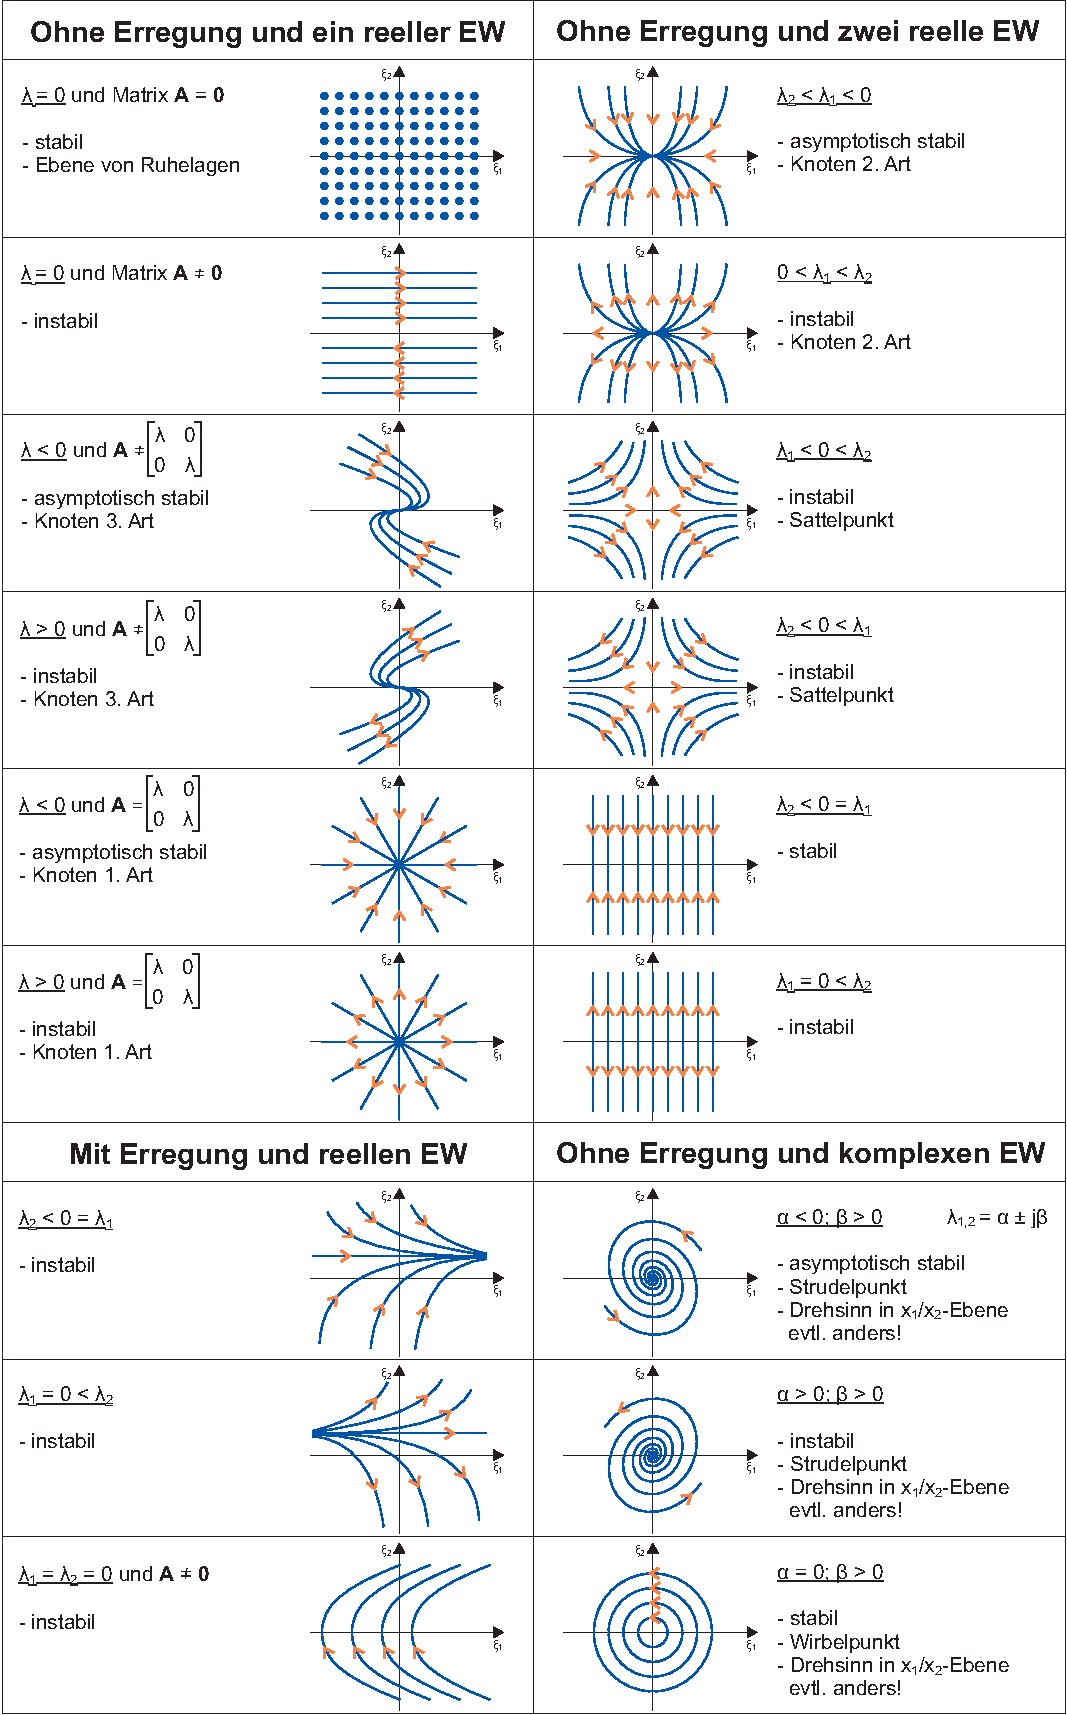
\includegraphics[width=0.85\textwidth]{Grafiken/Phasenportraits}
\end{center}
\end{figure*}

\end{document}








